
\chapter{Elemente der Stochastik}

\section{Grundbegriffe}

\subsection{Ereignisse}

Die Wahrscheinlichkeitstheorie beschäftigt sich mit
\emph{Zufallsexperimenten}. Darunter versteht man ein Experiment
mit zufälligem Ausgang, das, um der Wissenschaftlichkeit genüge zu tun,
unter genau definierten Versuchsbedingungen durchgeführt wird.
Der Ausgang führt immer zu einem \emph{Ergebnis}. Alle erreichbaren
Ergebnisse fasst man zur \emph{Ergebnismenge} zusammen. Allgemeiner
genügt es, wenn jedes Ergebnis in der Ergebnismenge liegt, wobei diese
aber auch Elemente enthalten darf, die das Experiment niemals abwirft.
Jede Teilmenge der Ergebnismenge nennt man ein \emph{Ereignis}\index{Ereignis}.
Die Potenzmenge der Ergebnismenge heißt \emph{Ereignisraum}, sie
besteht aus allen denkbaren Ereignissen. Man sagt, ein Ereignis sei
eingetreten, wenn das Ergebnis des Versuchs im diesem Ereignis liegt.

Zu beachten ist, dass wir dabei eine endliche oder höchstens
abzählbar unendliche Ergebnismenge voraussetzen. Bei überabzählbaren
Ergebnismengen kommt es zu Unwägbarkeiten, deren Klärung Gegenstand der
Maßtheorie ist.

Ein schlichtes Experiment bietet der Wurf des Spielwüfels, eines mit
Augenzahlen beschrifteten regelmäßigen Hexaeders. Die Ergebnismenge
wird als
\[\Omega := \{1, 2, 3, 4, 5, 6\}\]
festgelegt. Betrachten wir die drei Ereignisse
\[A := \{2\},\quad B := \{1,2\},\quad C:=\{1,3\}.\]
Ist $\omega=2$ das Ergebnis des Versuchs, sind die Ereignisse $A,B$
eingetreten. Zwei Ereignisse, die niemals gleichzeitig eintreten,
heißen \emph{disjunkt}. So sind die $A,C$ disjunkt, weil ihre
Schnittmenge leer ist.

\subsection{Nochmals Indikatorfunktionen}

In diesem Abschnitt will ich nochmals näher auf Indikatorfunktionen
eingehen. Sie bieten in der Kombinatorik und in der
Wahrscheinlichkeitsrechnung beim Rechnen mit Summen ein Hilfsmittel,
das bestimmte Umformungen leichter verständlich macht.

\begin{table}
\centering
\caption{Regeln für die Iverson-Klammerung}
\label{tab:Iverson}
\begin{tabular}{r@{\;}l@{\qquad}r@{\;}l}
\toprule
$[\bot]$ & $= 0$ & $[a\land b]$ & $= [a]\cdot [b]$\\
$[\top]$ & $= 1$ & $[a\lor b]$ & $= [a] + [b] - [a]\cdot [b]$\\
$[\lnot a]$ & $= 1 - [a]$ & $[a\oplus b]$ & $= |[a] - [b]|$\\
\bottomrule
\end{tabular}
\end{table}

Wir rekapitulieren nochmals die Iverson"=Klammerung, die Wahrheitswerte
in die Menge der Zahlen einbettet. Für jede Aussage $E$ ist
\[[A] := \begin{cases}
0, & \text{wenn $A$ falsch ist,}\\
1, & \text{wenn $A$ wahr ist.}
\end{cases}\]
Hiermit wird zu jeder Menge $M\subseteq\Omega$ die Indikatorfunktion als
\[1_M\colon\Omega\to\{0,1\},\quad 1_M(\omega) := [\omega\in M]\]
festgelegt. Für die Iverson"=Klammerung gelten die Regeln in Tabelle
\ref{tab:Iverson}, die man leicht per Wahrheitstafel nachrechnen kann.
Es wäre zu bemerken, dass man damit genau die Einbettung der
Aussagenlogik in die gewöhnliche Algebra erhält, wie Boole sie
darstellte.
\begin{Satz}\label{Indikatorf-Vereinigung2}
Für jedes $\omega$ gilt
\[1_{A\cup B}(\omega) = 1_A(\omega) + 1_B(\omega) - 1_{A\cap B}(\omega).\]
\end{Satz}
\begin{Beweis}
Laut Definition ist die Gleichung äquivalent zur Gleichung
\begin{align*}
&[\omega\in A\cup B] = [\omega\in A] + [\omega\in B] - [\omega\in A\cap B]\\
\iff & [\omega\in A\lor\omega\in B] = [\omega\in A] + [\omega\in B] - [\omega\in A\land\omega\in B].
\end{align*}
Diese gilt aber gerade laut Tabelle \ref{tab:Iverson}.\,\qedsymbol
\end{Beweis}

\noindent
Die Indikatorfunktion einer endlichen Mengen ermöglicht es, die
Anzahl ihrer Elemente als eine Summe darzustellen. Man sieht sofort ein,
dass $|A| = \sum_{\omega\in\Omega} 1_A(\omega)$ für eine Menge $A\subseteq\Omega$
gelten muss, was recht trivial erscheinen mag. Infolge erhält man aber aus
Satz \ref{Indikatorf-Vereinigung2} unverzüglich den Korollar
\[|A\cup B| = |A|+|B|-|A\cap B|.\]

\subsection{Wahrscheinlichkeiten}

Man kann nicht voraussagen, wie ein Experiment ausgehen wird. Das
Wahrscheinlichkeitsmaß liefert dennoch ein Maß dafür, wie sicher der
Eintritt eines Ereignisses ist. Wahrscheinlichkeit wird tiefergründig
verständlich, wenn dasselbe Zufallsexperiment abermals wiederholt wird.
Wir zählen, wie häufig ein Elementarereignis eingetreten ist.

Es sei ein Versuch $n$ mal durchgeführt worden, was zu den Ergebnissen
$a_i$ für $i=1$ bis $i=n$ geführt hat. Wir definieren die \emph{relative
Häufigkeit} des Ereignisses $A$ als die Zahl
\[r_{n,a}(A) := \frac{1}{n}|\{i\in\{1,\ldots,n\}\mid a_i\in A\}|.\]
Relative Häufigkeiten bieten bei hinreichend großem $n$ eine Näherung
für die Wahrscheinlichkeit. Zur Vermessung eines Würfels wird man
diesen also möglichst oft werfen wollen. Man erhält so die relativen
Häufigkeiten der Elementarereignisse, und damit näherungsweise auch
ihre Wahrscheinlichkeiten. So lässt sich feststellen, ob ein
Würfel gezinkt wurde.

Fassen wir $a$ als Funktion $i\mapsto a_i$ auf, können wir schreiben
\[\{i\mid a_i\in A\} = \{i\mid i\in a^{-1}(A)\} = a^{-1}(A).\]
Für disjunkte Ereignisse $A,B$ erhält man nun
\begin{align*}
r_{n,a}(A\cup B) &= \tfrac{1}{n}|a^{-1}(A\cup B)|
= \tfrac{1}{n}|a^{-1}(A)\cup a^{-1}(B)|\\
&= \tfrac{1}{n}|a^{-1}(A)| + \tfrac{1}{n}|a^{-1}(B)|
= r_{n,a}(A) + r_{n,a}(B).
\end{align*}
Weil $\Omega$ die Zielmenge von $a$ ist, muss $a_i\in\Omega$
für jedes $i\in\Omega$ gelten, also $|a^{-1}(\Omega)|=n$. Somit gilt
\[r_{n,a}(\Omega) = 1,\]
unabhängig davon, wie groß die Zahl $n$ ist. Und weil sich aus der
Definition von $a$ unmittelbar $0\le |a^{-1}(A)|\le n$ ergibt, besteht der
Sachverhalt
\[0\le r_{n,a}(A)\le 1.\]
Weiterhin ergibt sich, dass sich die Häufigkeit monoton bezüglich der
Inklusion verhält, das heißt, es besteht die Implikation
\[A\subseteq B\Rightarrow r_{n,a}(A)\le r_{n,b}(B).\]
Laut Satz \ref{Monotonie-Bild-Urbild} folgt nämlich $a^{-1}(A)\subseteq a^{-1}(B)$
aus $A\subseteq B$. Daraufhin ergibt sich $|a^{-1}(A)|\le |a^{-1}(B)|$.

Die Vorstellung von der Wahrscheinlichkeit besteht darin, dass sich
die relative Häufigkeit ihr mit steigender Anzahl der Versuche immer
weiter nähert. Dies bedeutet, es wird meistens $P(A)\approx r_{n,a}(A)$
für hinreichend großes $n$ gelten. Die bisher erläuterten Eigenschaften
von $r_{r,a}$ sollten diesbezüglich für $P$ bestehen bleiben, da diese
nicht von $n$ abhängen.

Untermauert wird diese Überlegung durch das \emph{Gesetz der großen
Zahlen}. Es zu diskutieren, würde an dieser Stelle aber zu weit führen.
Zum einem müsste dafür zunächst der Begriff des Grenzwertes eingeführt werden.
Zum anderen ist der Grenzwertbegriff der Analysis nicht in direkter
Weise auf den Sachverhalt anwendbar. Auf dessen Basis müssten zunächst
die Konvergenzbegriffe für Zufallsgrößen erörtert werden.

Stattdessen wird der Begriff des Wahrscheinlichkeitsmaßes erst einmal
axiomatisch eingeführt. Darauf aufbauend, was unter einer Zufallsgröße
zu verstehen sei.

\begin{Definition}[Endlicher Wahrscheinlichkeitsraum]\newlinefirst
Sei $\Omega$ eine nichtleere endliche Menge. Das Paar $(\Omega,P)$ nennt
man einen \emph{endlichen Wahrscheinlichkeitsraum}, wenn
\[P\colon\powerset(\Omega)\to\R,\quad P(A) := \sum_{\omega\in A}P(\{\omega\})\]
die Eigenschaften $\mathrm{Bild}(P) = [0,1]$ und $P(\Omega)=1$ besitzt.
\end{Definition}

\noindent
Ein endlicher Wahrscheinlichkeitsraum kann alternativ auch durch die
kolmogorowschen Axiome charakterisiert werden. Der Vorteil besteht darin,
dass diese später auch unter allgemeineren Umständen gültig bleiben.

\begin{Satz}[Axiome von Kolmogorow]\label{Axiome-Kolmogorow}\newlinefirst
Sei $\Omega$ eine nichtleere endliche Menge und
$P\colon\powerset(\Omega)\to\R$. Es ist $(\Omega,P)$ genau dann
ein endlicher Wahrscheinlichkeitsraum, wenn
\begin{align*}
& P(A) \ge 0\;\text{für}\;A\in\Omega,\\
& P(\Omega) = 1,\\
& P(A\cup B) = P(A) + P(B)\;\text{für}\;A,B\in\Omega\;
\text{mit}\;A\cap B=\emptyset.
\end{align*}
\end{Satz}
\begin{Beweis}
Es sei $(\Omega,P)$ ein endlicher Wahrscheinlichkeitsraum.
Mit $A\cap B=\emptyset$ gilt für die Indikatorfunktionen
gemäß Satz \ref{Indikatorf-Vereinigung2} die Gleichung
\[1_{A\cup B}(\omega) = 1_A(\omega) + 1_B(\omega).\]
Somit gelingt die Rechnung
\begin{gather*}
P(A\cup B) = \sum_{\omega\in A\cup B}P(\{\omega\})
= \sum_{\omega\in\Omega}P(\{\omega\})1_{A\cup B}(\omega)\\
= \sum_{\omega\in\Omega}P(\{\omega\})(1_A(\omega)+1_B(\omega))
= \sum_{\omega\in\Omega}P(\{\omega\})1_A(\omega)+
\sum_{\omega\in\Omega}P(\{\omega\})1_B(\omega)\\
= \sum_{\omega\in A}P(\{\omega\}) + \sum_{\omega\in B}P(\{\omega\})
= P(A) + P(B).
\end{gather*}
Umgekehrt erfülle $(\Omega,P)$ die kolmogorowschen Axiome. Da die
elementaren Ereignisse $\{\omega\}$ paarweise disjunkt sind, ergibt sich
\[P(A) = P(\bigcup_{\omega\in A}\{\omega\})
= \sum_{\omega\in A} P(\{\omega\}).\]
Mit dieser Summenformel erhält man die Aussage $P(A)\le 1$ nun als Korollar
aus Satz \ref{Monotonie-P} mit $A:=A$ und $B:=\Omega$.\,\qedsymbol
\end{Beweis}

\begin{Satz}\label{Monotonie-P}
Gilt $A\subseteq B$, so ist $P(A)\le P(B)$.
\end{Satz}
\begin{Beweis}
Mit $A\subseteq B$ ist $1_A(\omega)\le 1_B(\omega)$ für jedes $\omega\in\Omega$.
Ergo gilt
\[P(A) = \sum_{\omega\in\Omega} P(\{\omega\})1_A(\omega)
\le \sum_{\omega\in\Omega} P(\{\omega\})1_B(\omega) = P(B).\,\qedsymbol\]
\end{Beweis}

\noindent
Die Vorstellung von der Wahrscheinlichkeit als Chance oder Risiko
mag aufgrund ihres Charakters als Unwägbarkeit schwierig fassbar sein.
Der frequentistische Wahrscheinlichkeitsbegriff wird hingegen mit seiner
Erklärung von Wahrscheinlichkeit als relative Häufigkeit bei großer
Zahl der Versuche schon greifbarer. Mir fällt dazu eine Sichtweise ein,
die sich dem zufälligen Charakter so weit entzieht wie es nur geht.
Lässt man die große Zahl der Versuche parallel ablaufen, gibt die
die Wahrscheinlichkeit den \emph{Anteil} der Ergebnisse an, die in
der jeweiligen Teilmenge enthalten sind. Werdem zum Beispiel eine
Million Spielwürfel auf einmal geworfen, wird jede der Augenzahlen
voraussichtlich näherungsweise mit dem Anteil $\frac{1}{6}$ vorkommen.
Oder denkt man sich eine Population von unzählig vielen Individuen,
und erhält jedes die gleiche Wahrscheinlichkeit $P(A)$, ein
bestimmtes Merkmal $A$ zu besitzen, wird man in der Population einen
Anteil von näherungsweise $P(A)$ Individuen mit dem Merkmal $A$ vorfinden.

Das Wahrscheinlichkeitsmaß $P$ erfüllt einige Gesetzmäßigkeiten, die
elementar aus den Axiomen ableitbar sind.

\begin{Satz}
Allgemein gilt $P(A^\compc) = 1 - P(A)$.
\end{Satz}
\begin{Beweis}
Da $\Omega = A\cup A^\compc$ eine Zerlegung von $\Omega$ in zwei
disjunkte Mengen ist, erhält man $P(\Omega)=P(A)+P(A^\compc)$.
Die Gleichung $P(\Omega)=1$ wird daraufhin kurzum nach $P(A^\compc)$
umgeformt.\,\qedsymbol
\end{Beweis}

\begin{Satz}\label{Inklusion-Exklusion-zwei}
Allgemein gilt $P(A\cup B) = P(A) + P(B) - P(A\cap B)$.
\end{Satz}
\begin{Beweis}
Vermittels Satz \ref{Indikatorf-Vereinigung2} formt man wie im Beweis
von Satz \ref{Axiome-Kolmogorow} die Summenformel für
$P(A\cup B)$ um.\,\qedsymbol
\end{Beweis}

\noindent
Alternativ kann die Identität folgendermaßen direkt aus dem dritten
kolmogorowschen Axiom abgeleitet werden, ohne den Weg über die Summenformel
zu gehen. Man überzeugt sich mühelos davon, dass $A$ via%
\[A = A\cap\Omega = A\cap(B\cup B^\compc) = (A\cap B)\cup (A\cap B^\compc)\]
als Vereinigung disjunkter Mengen dargestellt werden kann. Ergo gilt%
\[P(A) = P(A\cap B) + P(A\cap B^\compc).\]
Analog bekommt man
\[A\cup B = (A\cup B)\cap (B\cup B^\compc) =
((A\cup B)\cap B)\cup ((A\cup B)\cap B^\compc)\]
als Vereinigung disjunkter Mengen. Der letzte Term vereinfacht sich
mit dem Absorptionsgesetz $(A\cup B)\cap B = B$ und $(A\cup B)\cap B^\compc
= A\cap B^\compc$ via Distributivgesetz, Komplementärgesetz und
Neutralitätsgesetz. Demzufolge gilt%
\[P(A\cup B) = P(B) + P(A\cap B^\compc).\]
Löst man die vorherige Gleichung nun nach $P(A\cap B^\compc)$ auf
und setzt sie in diese ein, findet sich schließlich Satz
\ref{Inklusion-Exklusion-zwei}.

Vermittels Satz \ref{Inklusion-Exklusion-zwei} wird unschwer die Formel
\[P(A\cup B\cup C) = P(A) + P(B) + P(C)
- P(A\cap B) - P(A\cap C) - P(B\cap C) + P(A\cap B\cap C)\]
gewonnen. Umgekehrt kann Satz \ref{Inklusion-Exklusion-zwei} unmittelbar
aus ihr zurückgewonnen werden, indem einfach $C:=\emptyset$ gesetzt
wird. Diese Formeln folgen einem allgemeinen Prinzip, das
allgemein für Vereinigungen endlich vieler Mengen gilt, -- man spricht
von der \emph{Siebformel}, auch als \emph{Prinzip der Inklusion und Exklusion}
geläufig.

\subsection{Gleichverteilungen}

Viele Zufallsexperimente entstehen aus einer Zusammensetzung vermittels
Gegenständen, die einer Gleichverteilung unterliegen, wo also jedes der
elementaren Ereignisse gleich wahrscheinlich ist. Zum Beispiel ist dies
beim Wurf einer idealen Münze, beim Wurf eines idealen Würfels, bei
der Ziehung einer Karte aus einem gut durchmischten Stapel nummerierter
Karten oder bei der Ziehung einer Kugel aus einer Ansammlung nummerierter
Kugeln der Fall. Auch ein Zufallszahlgenerator mit einer bestimmten Verteilung
lässt sich vermittels bestimmter Algorithmen aus einem gleichverteilten
Generator aufbauen.

Wir nehmen nun für eine Weile die Position ein, dass auf unterster Ebene
immer eine Gleichverteilung herrscht. Wie sich herausstellt, ist diese
These unhaltbar. Das ist aber nicht weiter schlimm, denn auch dieser
eingeschränkte Wahrscheinlichkeitsbegriff zeigt sich bisweilen recht
vielfältig.

\begin{Definition}[Laplace-Experiment]\newlinefirst
Ein \emph{Laplace-Experiment} ist ein Zufallsexperiment, bei dem die
elementaren Ereignisse alle gleich wahrscheinlich sind.
\end{Definition}

\noindent
Der Wahrscheinlichkeitsraum $(\Omega,P)$ eines Laplace"=Experiments
hat also die Eigenschaft $P(\{\omega\})=c$ für jedes $\omega\in\Omega$,
wobei $c$ eine Konstante ist.

\begin{Satz}
Herrscht in $(\Omega,P)$ Gleichverteilung, gilt $P(A) = \frac{|A|}{|\Omega|}$.
\end{Satz}
\begin{Beweis}
Man stellt das Ereignis $A$ als Vereinigung der disjunkten elementaren
Ereignisse dar. Diesbezüglich ergibt sich die Umformung
\[P(A) = P(\bigcup_{\omega\in A}\{\omega\})
= \sum_{\omega\in A}P(\{\omega\}) = \sum_{\omega\in A} c
= c\sum_{\omega\in A} 1 = c\cdot |A|.\]
Speziell gilt $1=P(\Omega)=c\cdot |\Omega|$, womit
$c=\frac{1}{|\Omega|}$ sein muss.\,\qedsymbol
\end{Beweis}

\subsection{Zufallsgrößen}

Eine \emph{Zufallsgröße}\index{Zufallsgroesse@Zufallsgröße} darf man
sich als eine Funktion $X\colon\Omega\to\Omega'$
vorstellen, die eine kausale Verbindung zwischen den Ergebnismengen
$\Omega,\Omega'$ schafft. Ein Ergebnis $\omega\in\Omega$ führt
zu $X(\omega)$. Ursächlich für ein $x\in\Omega'$ sind daher all die
$\omega$ mit $x=X(\omega)$. Das heißt, ursächlich für das
Elementarereignis $\{x\}$ ist dessen Urbild $X^{-1}(\{x\})$.
Infolge muss die Wahrscheinlichkeit von $\{x\}$ die es Urbildes sein.
Insofern definiert man auf $\Omega'$ das Wahrscheinlichkeitsmaß%
\[P_X\colon\mathcal P(\Omega')\to [0,1],\quad P_X(A) := P(X^{-1}(A)).\]
Man nennt $P_X$ die \emph{Verteilung}\index{Verteilung} von $X$. Mit der
identischen Zufallsgröße
\[\id\colon\Omega\to\Omega,\quad \id(\omega) := \omega\]
versteht sich auch das ursprüngliche Maß $P$ als die Verteilung $P=P_{\id}$.

Geläufig sind die Schreibweisen
\begin{align*}
P(X=x) &:= P(X^{-1}(\{x\})), & \{X=x\} &:= X^{-1}(\{x\}),\\
P(X\in A) &:= P(X^{-1}(A)), & \{X\in A\} &:= X^{-1}(A).
\end{align*}
Es ist $\{X=x\}$ dasselbe wie $\{X\in\{x\}\}$. 
Ist $P$ die Gleichverteilung auf $\Omega$, ergibt sich
\[P(X\in A) = \frac{|\{X\in A\}|}{|\Omega|}.\]
Standardbeispiel. Wir werfen zwei Spielwürfel.
Die Ergebnismenge sei%
\[\Omega := \{1,\ldots,6\}\times\{1,\ldots,6\},\]
und jedes der 36 elementaren Ereignisse sei gleich wahrscheinlich, habe
also die Wahrscheinlichkeit $\tfrac{1}{36}$.
Es bezeichne $\omega_1$ das Ergebnis des ersten, und $\omega_2$
das des zweiten Wurfs. Wir betrachten die Zufallsgröße%
\[X\colon\Omega\to\{2,\ldots,12\},\quad
X(\omega_1,\omega_2) := \omega_1+\omega_2.\]
Gesucht sei $P(X=4)$. Man ermittelt
\[\{X=4\} = \{(1,3), (2,2), (3,1)\},\quad\text{ergo}\;P(X=4) = \tfrac{3}{36}.\]
Allgemein zerfällt ein Ereignis $A$ ja in seine disjunkten Elementarereignisse
$\{x\}$, so dass $A = \bigcup_{x\in A} \{x\}$ gilt. Weil nun die
Fasern $X^{-1}(\{x\})$ ebenfalls disjunkt sind, muss $P(X\in A)$ die
Summe der $P(X=x)$ mit $x\in A$ sein. Das heißt, man rechnet%
\[P(X\in A) = P(X^{-1}(\bigcup_{x\in A} \{x\})) = P(\bigcup_{x\in A} X^{-1}(\{x\}))
= \sum_{x\in A} P(X=x).\]
Die Verteilung $P_X$ ist demzufolge bereits eindeutig bestimmt,
sobald $P(X=x)$ für jedes $x\in\Omega'$ vorliegt. Dies motiviert
uns, die Funktion
\[p_X\colon\Omega\to[0,1],\quad p_X(x) := P(X=x)\]
zu definieren, genannt die \emph{Wahrscheinlichkeitsfunktion} der
Zufallsgröße $X$.

\newpage
\section{Bedingte Wahrscheinlichkeiten}

\subsection{Mehrstufige Experimente}

Es findet ein zweistufiges Experiment statt, welches sich sich
aus einem ersten und einem zweiten Wurf eines Spielwürfels
zusammensetzt. Bei jedem der Würfe bestehe eine Gleichverteilung.
Zur Frage steht, wie wahrscheinlich das Ereignis $\{(6,6)\}$ ist.
Ein Paar $(\omega_1,\omega_2)$ fasse hierbei das Ergebnis $\omega_1$
des ersten und $\omega_2$ des zweiten Wurfs zusammen.

Die Wahrscheinlichkeit der ersten Sechs beträgt $\tfrac{1}{6}$,
die der zweiten ebenfalls $\tfrac{1}{6}$. Sie multiplizieren sich
zu $\tfrac{1}{36}$, richtig?

Es wäre doch möglich, dass zwischen den beiden Würfen eine,
sagen wir, geisterhafte Beziehung besteht, dergestalt dass
der zweite Wurf niemals in einer Sechs resultiert, sofern das
Ergebnis des ersten eine war. Trotzdem sind die Wahrscheinlichkeiten bei
jedem der Würfe für sich allein gesehen gleichverteilt. Dafür muss man
nicht unbedingt die Wirklichkeit manipulieren. Das Phänomen ist bereits
bei der Erzeugung von Zufallszahlen im Computer beobachtbar. War die
erste Zufallszahl eine Sechs, braucht der Generator die zweite lediglich
solange zu verwerfen, wie sie eine Sechs sein sollte. Umstände dieser
Art stellen nicht nur ein Gedankenspiel dar, so dass wir uns notgedrungen
mit ihnen auseinandersetzen müssen. Sie führen zum Begriff der
\emph{bedingten Wahrscheinlichkeit}.

Bisher wurde immer nur die Verteilung der Wahrscheinlichkeiten eines
Würfels für sich allein betrachtet. Das war modelliert durch die Größe
\[X_0\colon\Omega\to\Omega,\quad X_0(\omega):=\omega,\quad \Omega := \{1,\ldots,6\},\]
mit der Gleichverteilung $P_0$, so dass $P_0(X=6)=\tfrac{1}{6}$.

Wir modellieren das zweistufige Experiment durch die Zufallsgröße
\[X\colon\Omega^2\to\Omega^2,\quad X(\omega) := (X_1,X_2)(\omega)
= (X_1(\omega), X_2(\omega)),\]
die sich mit $\omega = (\omega_1,\omega_2)$ aus den zwei Zufallsgrößen
\begin{gather*}
X_1\colon\Omega^2\to\Omega,\quad X_1(\omega_1,\omega_2) := \omega_1,\\
X_2\colon\Omega^2\to\Omega,\quad X_2(\omega_1,\omega_2) := \omega_2
\end{gather*}
zusammensetzt. Es stellt $X_1(\omega)$ das Ergebnis des ersten und
$X_2(\omega)$ das des zweiten Wurfs dar. Wie gewünscht gilt
\[(X_1(\omega),X_2(\omega)) = (X_0(\omega_1),X_0(\omega_2)) = (\omega_1,\omega_2).\]
Es bezeichne $P$ die Verteilung auf $\Omega^2$. Wir wissen hier allerdings
lediglich
\begin{gather*}
P(X_1=\omega_1) = P_0(X_0=\omega_1) = \tfrac{1}{6},\\
P(X_2=\omega_2) = P_0(X_0=\omega_2) = \tfrac{1}{6}.
\end{gather*}
Die Fehlannahme besteht nun darin, dass per se
\[P(\{X_1=\omega_1\}\cap\{X_2=\omega_2\}) = P(X_1=\omega_1)P(X_2=\omega_2)\]
gelten müsse. Ist diese Gleichung erfüllt, nennt man die
Zufallsgrößen $X_1,X_2$ \emph{unabhängig}. In der bisherigen Sichtweise,
wo wir nur $X_0$ mit $P_0$ gesehen haben, war es uns nicht möglich,
stochastische Abhängigkeit zu beschreiben. Man notiert allgemein%
\[P(X=x,Y=y) := P(\{X=x\}\cap\{X=y\}) = P(X=x)P(Y=y\mid X=x).\]
Der letzte Faktor bezeichne hierbei die bedingte Wahrscheinlichkeit
für das Ereignis $\{Y=y\}$, unter der Bedingung, dass $\{X=x\}$
bereits eingetreten ist.
\begin{Definition}[Bedingte Wahrscheinlichkeit]\newlinefirst
Die \emph{bedingte Wahrscheinlichkeit} für den Eintritt von $A$ unter
der Bedingung $B$ ist für $P(B)\ne 0$ definiert gemäß
\[P(A\mid B) := \frac{P(A\cap B)}{P(B)}.\]
\end{Definition}
Wir setzen speziell $B:=\{X=x\}$ und $A:=\{Y=y\}$ ein,
das macht
\[P(Y=y\mid X=x) = \frac{P(X=x,Y=y)}{P(X=x)}.\]
Sind $X,Y$ unabhängig, gilt also
\[P(Y=y\mid X=x) = P(Y=y).\]
Mit der geisterhaften Beziehung zwischen den Würfeln wäre allerdings
\[0 = P(X_2=6\mid X_1=6) \ne P(X_1=6) = \tfrac{1}{6}.\]
Reflektiert man den Begriff der bedingten Wahrscheinlichkeit
eingehend, fällt auf, dass dieser nicht zwangsläufig ein mehrstufiges
Experiment voraussetzt. Zugleich kann ein zweistufiges Experiment auch
als einstufiges mit Paaren als Ergebnissen interpretiert werden. Zur
Verdeutlichung will ich die bedingte Wahrscheinlichkeit aber nochmals
bei einem eigentlich einstufigen Experiment diskutieren. Es wird
einmalig ein gewöhnlicher Würfel geworfen, die Wahrscheinlichkeit für das
Ereignis $\{4\}$ beträgt offenkundig $\frac{1}{6}$. Es sei nun $B$ das
Ereignis, dass eine gerade Zahl geworfen wurde. Diesbezüglich ergibt sich
\[P(\{4\}\mid B) = \frac{P(\{4\}\cap B)}{P(B)} = \frac{P(\{4\})}{1/2}
= 2\cdot\frac{1}{6} = \frac{1}{3}.\]
Dieser Umstand mag intuitiv begreiflich sein. Wenn bereits bekannt
ist, dass eine gerade Zahl geworfen wurde, verbleiben nur noch drei
Möglichkeiten für das Ergebnis, womit jedes der drei zugehörigen
elementaren Ereignisse, die anscheinend gleichberechtigt sind, die
Wahrscheinlichkeit $\frac{1}{3}$ besitzen muss.

Bei einem mehrstufigen Zufallsexperiment stellt das \emph{Baumdiagramm} ein
Hilfsmittel zur Schaffung von Übersicht dar. An ihm wird die erste
und zweite Pfadregel ersichtlich gemacht. Wir betrachten dazu zunächst
ein zweistufiges Experiment mit der Ergebnismenge $\Omega =
\Omega_1\times\Omega_2$. Ist $a\in\Omega$ mit $a=(a_1,a_2)$ das Ergebnis
des Experiments, so ist $a_1\in\Omega$ das erste Teilergebnis. Es stellt
sich zunächst einmal die Frage, wie die Wahrscheinlichkeit zu diesem
ausgedrückt wird, wo $P$ eigentlich auf $\Omega$ definiert ist,
nicht aber auf $\Omega_1$. Sie muss gleich $P(\{a_1\}\times\Omega_2)$
sein, insofern das zweite Ergebnis noch unbekannt verbleibt, also
keine Rolle spielen darf. Nun würde man analog sagen, das zweite Ergebnis
besäße die Wahrscheinlichkeit $P(\Omega_1\times\{a_2\})$, aber das
kann so nicht allgemein stimmen, denn die Wahrscheinlichkeit zu $a_2$
ist unter Umständen vom Ausgang des ersten Teilexperiments abhängig.
Zur Abkürzung sei $B:=\{a_1\}\times\Omega_2$ und $A:=\Omega_1\times\{a_2\}$.
Wenn die Wahrscheinlichkeit vom Ausgang zu $a_2$ gewünscht ist, bei
der $a_1$ bereits eingetreten ist, handelt es sich nicht um $P(A)$,
sondern um $P(A\mid B)$. Man rechnet diesbezüglich
\[P(\{a\}) = P(B\cap A) = P(B)P(A\mid B).\]
Die ist die \emph{erste Pfadregel}.\index{Pfadregel, erste} Sie besagt,
dass die Wahrscheinlichkeit eines elementaren Ereignisses gleich dem
Produkt der Wahrscheinlichkeiten entlang des Pfades ist, der zu diesem
Ereignis führt.

\strong{Beispiel.} In einer Urne befinden sich eine weiße und
drei schwarze Kugeln. Es werden zwei Kugeln gezogen, wobei ihre
Reihenfolge von Belang sei. Gesucht ist die Wahrscheinlichkeit der
elementaren Ereignisse. Die Abb. \ref{fig:Baumdiagramm-Urne} zeigt das
Baumdiagramm zu diesem Experiment. Wir haben hier die Erbebnismenge
\[\Omega = \Omega_1\times\Omega_2 = \{\bullet,\circ\}\times\{\bullet,\circ\}
= \{(\bullet,\bullet),(\bullet,\circ),(\circ,\bullet),(\circ,\circ)\}.\]
Zu $B := \{\bullet\}\times\Omega_2$ und $A := \Omega_1\times\{\circ\}$
ergibt sich
\[P(\{(\bullet,\circ)\}) = P(B)P(A\mid B) = \tfrac{3}{4}\cdot\tfrac{1}{3} = \tfrac{1}{4}.\]

\begin{figure}\setlength{\abovecaptionskip}{0pt}
\begin{center}
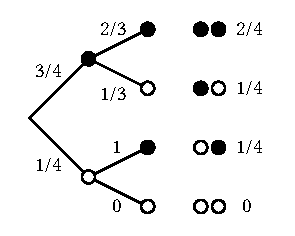
\includegraphics[width=50mm]{img/Baumdiagramm-Urne.pdf}
\caption{Baumdiagramm zur Ziehung aus der Urne}
\label{fig:Baumdiagramm-Urne}
\end{center}
\end{figure}

\noindent
Um die erste Pfadregel für Experimente mit mehr als zwei Stufen bestätigen
zu können, müssen wir zunächst ein paar Vorbetrachtungen machen.
Zunächst wird sich die Frage auftun, wie man bedingte Wahrscheinlichkeiten
von bedingten Wahrscheinlichkeiten bildet. Bei fester Bedingung $B$
bildet die bedingte Wahrscheinlichkeit wiederum ein Wahrscheinlichkeitsmaß,%
\[P_B\colon\Omega\to\R,\quad P_B(A) := P(A\mid B).\]
Diesbezüglich kann man nun von $P_B(A\mid C)$ reden. Allerdings findet
sich hierzu die Umformung%
\[P_B(A\mid C) = \frac{P_B(A\cap C)}{P_B(C)}
= \frac{\frac{P(A\cap B\cap C)}{P(B)}}{\frac{P(B\cap C)}{P(B)}}
= \frac{P(A\cap B\cap C)}{P(B\cap C)} = P(A\mid B\cap C).\]
Das heißt, die Schachtelung von bedingten Wahrscheinlichkeiten stimmt
mit der bedingten Wahrscheinlichkeit unter konjunktiver Verbindung der
Bedingungen, ausgedrückt als Schnittmenge, überein. Für $P(A\mid B\cap C)$
ist auch die Schreibweise $P(A\mid B,C)$ geläufig.

\subsection{Gesetz der totalen Wahrscheinlichkeit}

\begin{Satz}[Gesetz der totalen Wahrscheinlichkeit]\newlinefirst
Es sei $\setsystem Z$ eine Zerlegung der Ergebnismenge $\Omega$ in
paarweise disjunkte Mengen $B\in\setsystem Z$. Dann gilt
\[P(A) = \sum_{B\in\setsystem Z}P(A\mid B)P(B).\]
\end{Satz}
\begin{Beweis}
Es findet sich die Umformung
\begin{align*}
P(A) &= \textstyle P(A\cap\Omega) = P(A\cap\bigcup_{B\in\setsystem Z} B)
= P(\bigcup_{B\in\setsystem Z} (A\cap B))\\
&=\textstyle\sum_{B\in\setsystem Z} P(A\cap B)
= \sum_{B\in\setsystem Z} P(A\mid B)P(B).\,\qedsymbol
\end{align*}
\end{Beweis}
